
% This LaTeX was auto-generated from MATLAB code.
% To make changes, update the MATLAB code and republish this document.

\documentclass{article}
\usepackage{graphicx}
\usepackage{color}

\sloppy
\definecolor{lightgray}{gray}{0.5}
\setlength{\parindent}{0pt}

\begin{document}

    
    
\subsection*{Contents}

\begin{itemize}
\setlength{\itemsep}{-1ex}
   \item \% (1) Main Setup (folder handling)
   \item \% (2) Select Data
   \item (3.0) Test \#0 Quadprog vs Pure Lagrange
   \item (3.1) Test Sharpe Optimization
   \item (3.2) Compute Optimal Portfolio
\end{itemize}


\subsection*{\% (1) Main Setup (folder handling)}

\begin{verbatim}
clear
clc

HomeDir = 'F:/Mean-Value-Opt/';%<<<<-----Put your home directory
cd(strcat(HomeDir,'implementation'));

% Load all "background" data
[folders, dates, sectors] = dataLoc_retma(HomeDir);

% Inputs
RFR = [0.0365    0.0117    0.0143    0.0169    0.0100 ];%Bond Rates from Stats Canada
\end{verbatim}


\subsection*{\% (2) Select Data}

\begin{verbatim}
date   = dates(ceil(rand()*length(dates)));% select a random date
sector = sectors(ceil(rand()*length(sectors)));% select a random sector
[ Ret, CoRisk, stockNames, selData, data  ] = data_selector( folders, date, sector );
clc
fprintf('Loading %s Sector, from date %s-%s\n',...
    sector{:},date{:},num2str(str2num(date{:})+1));
\end{verbatim}

        \color{lightgray} \begin{verbatim}Loading Healthcare Sector, from date 2012-2013
\end{verbatim} \color{black}
    

\subsection*{(3.0) Test \#0 Quadprog vs Pure Lagrange}

\begin{verbatim}
clear mp n S M w WW
clc
mp  = 0.05;
n   = length(Ret);
S   = CoRisk(1:n,1:n);
M   = Ret(1:n);

% Matlab
tic
    w = quadprog(2.*S,[],[],[],[ M ; ones(1,n)],[mp;1],...
            [],[],[],...
            optimoptions('quadprog','Algorithm','interior-point-convex','Display','off'));
    fprintf('Matlab Time:  ');
toc

% Us
tic
    WW = [ 2*S M' ones(n,1); M 0 0 ; ones(1,n) 0 0 ]\[ zeros(n,1); mp; 1 ];
    fprintf('\nUs Time:  ');
toc

% Comparison
square_root_sum_of_error_squared = sqrt(sum((WW(1:end-2)-w).^2)./n)
\end{verbatim}

        \color{lightgray} \begin{verbatim}Matlab Time:  Elapsed time is 0.010595 seconds.

Us Time:  Elapsed time is 0.001041 seconds.

square_root_sum_of_error_squared =

   2.1231e-13

\end{verbatim} \color{black}
    

\subsection*{(3.1) Test Sharpe Optimization}

\begin{verbatim}
clear n M S rfr WMp mLims
clc
n       = 10;
tP      = 1:n;
M       = Ret(tP);
S       = CoRisk(tP,tP);
rfr     = RFR(1);
mLims   = 1E10;

% Matlab
tic
    p =  Portfolio('AssetMean',M,'AssetCovar',S,'RiskFreeRate',rfr,'Budget',1,'LowerBound',-mLims,'UpperBound',mLims);
    WMp = estimateMaxSharpeRatio(p);
    Matlab_Sharpe = (M*WMp-rfr)/sqrt(WMp'*S*WMp)
    fprintf('Matlab Time:  ');
toc
% Us
tic
    [ sharpe, Wp, ~, ~ ] = optimizeSupreme( M, S, rfr );
    Our_Sharpe = (M*Wp-rfr)/sqrt(Wp'*S*Wp)
    fprintf('\nUs Time:  ');
toc

disp(WMp./Wp);
\end{verbatim}

        \color{lightgray} \begin{verbatim}
Matlab_Sharpe =

    0.1680

Matlab Time:  Elapsed time is 0.773125 seconds.

Our_Sharpe =

    0.0871


Us Time:  Elapsed time is 0.102026 seconds.
   1.0e+08 *

    7.4242
    6.5300
    8.1999
    9.0027
    8.2916
    8.6679
    8.6131
    8.5564
    8.5252
    9.4506

\end{verbatim} \color{black}
    \begin{par}
Plots
\end{par} \vspace{1em}
\begin{verbatim}
figure('Name','Our Optimization');
    plot(Wp'*selData(:,1:n)');
    title('Our Function');
    xlabel('Time');
    ylabel('Value of Portfolio');
figure('Name','Matlab Optimization');
    plot(WMp'*selData(:,1:n)');
    xlabel('Time');
    ylabel('Value of Portfolio');
    title('Matlab');
\end{verbatim}

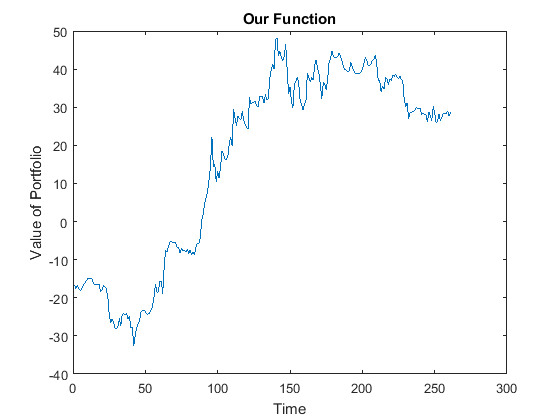
\includegraphics [width=4in]{compare_to_matlab_01.png}

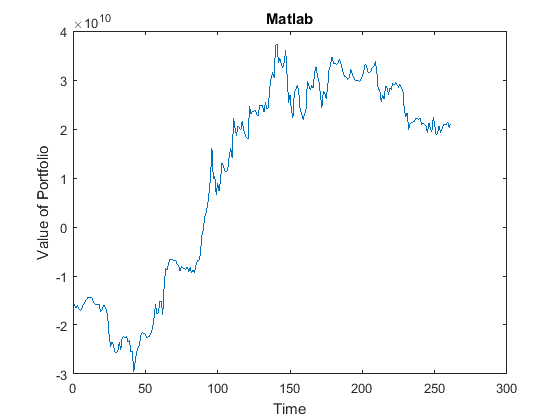
\includegraphics [width=4in]{compare_to_matlab_02.png}


\subsection*{(3.2) Compute Optimal Portfolio}

\begin{verbatim}
clc
n               = 20;
PortfolioLimit  = 10;
tic
    [ WpL, P, sharpe ] = optimizeSelect( Ret(1:n), CoRisk(1:n,1:n), RFR(1), PortfolioLimit )
toc
figure('Name',sprintf('Optimal %d Asset Portfolio', PortfolioLimit));
plot(WpL'*selData(:,P)');
\end{verbatim}

        \color{lightgray} \begin{verbatim}
WpL =

    4.9759
   -2.0228
   -2.0284
    3.5839
   -1.3225
    2.0891
   -4.0310
   -1.6807
    2.7206
   -1.2842


P =

     5     8     9    11    12    13    17    19    20    16


sharpe =

    0.1687

Elapsed time is 7.982953 seconds.
\end{verbatim} \color{black}
    
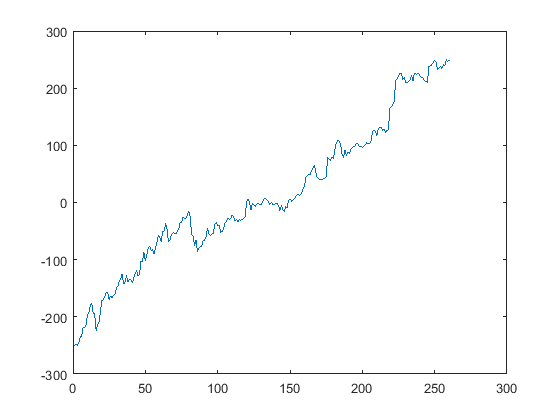
\includegraphics [width=4in]{compare_to_matlab_03.png}



\end{document}
    
